\section{Tài nguyên}
\subsection{Nguồn dữ liệu}
% hoang
Tập dữ liệu được sử dụng trong nghiên cứu này được lấy từ \underline{\url{https://finance.yahoo.com/}}, một nền tảng tài chính uy tín được biết đến với thông tin thị trường toàn diện và cập nhật. Tập dữ liệu bao gồm dữ liệu giá cổ phiếu của ba ngân hàng nổi tiếng tại Việt Nam: Ngân hàng Đầu tư và Phát triển Việt Nam (BIDV), Ngân hàng Thương mại Cổ phần Xuất Nhập Khẩu Việt Nam (Eximbank) và Ngân hàng Thương mại Cổ phần Ngoại Thương Việt Nam (Vietcombank). Bằng cách tận dụng dữ liệu có sẵn trên nền tảng này, chúng tôi đảm bảo một nền tảng đáng tin cậy cho phân tích của mình. Tập dữ liệu bắt đầu từ ngày 1 tháng 3 năm 2019 đến ngày 1 tháng 3 năm 2024, cung cấp một phạm vi thời gian mạnh mẽ cho phân tích của chúng tôi. Mỗi mục trong tập dữ liệu bao gồm các chỉ số tài chính chính, bao gồm:
\begin{itemize}
\item \textbf{Date}: Ngày giao dịch.
\item \textbf{Open}: Giá cổ phiếu mở cửa vào đầu ngày giao dịch.
\item \textbf{High}: Giá cổ phiếu cao nhất ghi nhận được trong ngày giao dịch.
\item \textbf{Low}: Giá cổ phiếu thấp nhất ghi nhận được trong ngày giao dịch.
\item \textbf{Close}: Giá cổ phiếu đóng cửa vào một ngày nhất định.
\item \textbf{Adj Close}: Giá đóng cửa được điều chỉnh, bao gồm bất kỳ hành động doanh nghiệp nào như cổ tức hoặc chia cổ phiếu.
\item \textbf{Volume}: Khối lượng giao dịch, chỉ ra tổng số cổ phiếu được giao dịch vào một ngày cụ thể.
\end{itemize}
\subsection{Thống kê mô tả}
\begin{table}[H]
    \centering
    \caption{Thống kê mô tả}
    \begin{tabular}{|c|c|c|c|}
         \hline
         \rowcolor{cyan}\centering\  & BIDV & Eximbank & Vietcombank\\\hline
         \multirow{1}{*}{Count} & 1306 & 1306 & 1306 \\\hline
         \multirow{1}{*}{Mean} & 33335.27142 & 16673.73704 & 66674.47299 \\\hline
         \multirow{1}{*}{Std} & 7058.435047 & 4257.231701 & 13618.83797 \\\hline
         \multirow{1}{*}{Min} & 21590.11133 & 10346.04492 & 37957.3125 \\\hline
         \multirow{1}{*}{Q1} & 28292.92188 & 12394.06738 & 56604.17578 \\\hline
         \multirow{1}{*}{Q2} & 31397.38281 & 16949.15234 & 65164.47656 \\\hline
         \multirow{1}{*}{Q3} & 38601.47266 & 19385.59375 & 75508.04297 \\\hline
         \multirow{1}{*}{Max}  & 54400 & 29661.01758  & 97400 \\\hline
         \multirow{1}{*}{Mode} & 28222.36719 & 12146.89258 & 55077.91797 \\\hline
         \multirow{1}{*}{Median} & 31397.38281 & 16949.15234 & 65164.47656 \\\hline
         \multirow{1}{*}{Var} & 49821505.31 & 18124021.75 & 185472747.7 \\\hline
         \multirow{1}{*}{Kurtosis} & 0.23806089 & -0.807813649 & -0.610997452 \\\hline
         \multirow{1}{*}{Skewness} & 0.840622466 & 0.442884414 & 0.336313457 \\\hline
         \multirow{1}{*}{CV} & 0.21174074 & 0.255325587 & 0.204258652 \\\hline
    \end{tabular}
    \label{descriptive-stats}
\end{table}

\begin{figure}[H]
    \centering
    \begin{minipage}{0.23\textwidth}
    \centering
    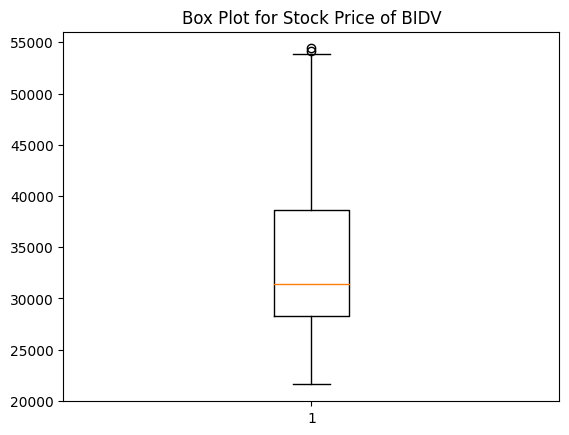
\includegraphics[width=1\textwidth]{resources/chapter-3/newdata/Boxplot_BIDV.png}
    \caption{BIDV stock price's boxplot}
    \label{fig:bidv_boxplot}
    \end{minipage}
    \hfill
    \begin{minipage}{0.23\textwidth}
    \centering
    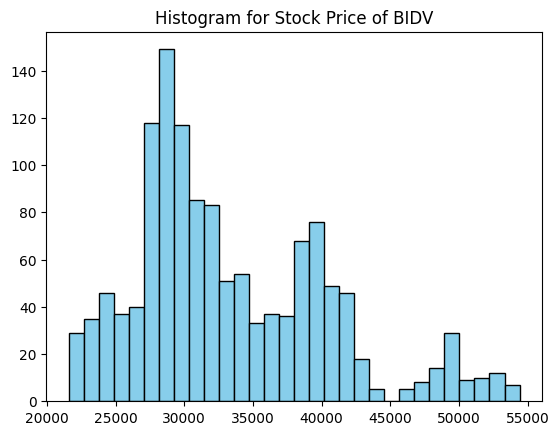
\includegraphics[width=1\textwidth]{resources/chapter-3/newdata/Histogram_BIDV.png}
    \caption{BIDV stock price's histogram}
    \label{fig:bidv_histogram}
    \end{minipage}
\end{figure}

\begin{figure}[H]
    \centering
    \begin{minipage}{0.23\textwidth}
    \centering
    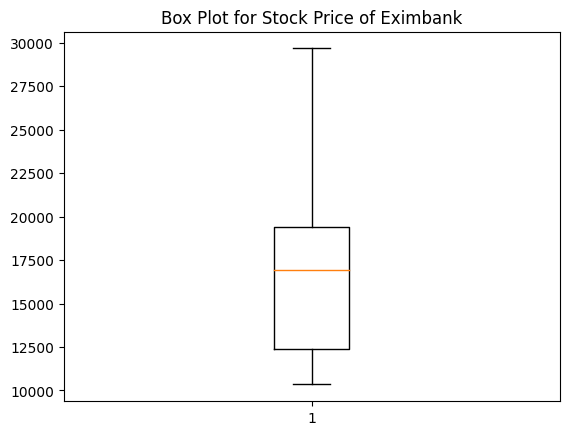
\includegraphics[width=1\textwidth]{resources/chapter-3/newdata/Boxplot_Eximbank.png}
    \caption{Eximbank stock price's boxplot}
    \label{fig:eximbank_boxplot}
    \end{minipage}
    \hfill
    \begin{minipage}{0.23\textwidth}
    \centering
    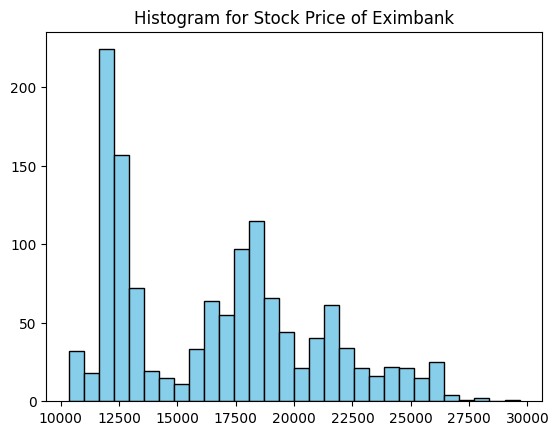
\includegraphics[width=1\textwidth]{resources/chapter-3/newdata/Histogram_Eximbank.png}
    \caption{Eximbank stock price's histogram}
    \label{fig:eximbank_histogram}
    \end{minipage}
\end{figure}

\begin{figure}[H]
    \centering
    \begin{minipage}{0.23\textwidth}
    \centering
    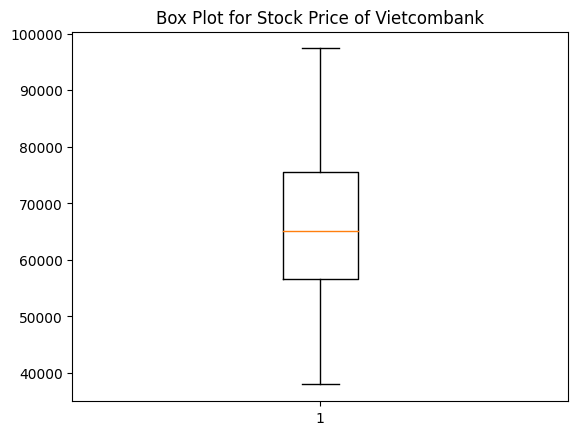
\includegraphics[width=1\textwidth]{resources/chapter-3/newdata/Boxplot_Vietcombank.png}
    \caption{VCB stock price's boxplot}
    \label{fig:vcb_boxplot}
    \end{minipage}
    \hfill
    \begin{minipage}{0.23\textwidth}
    \centering
    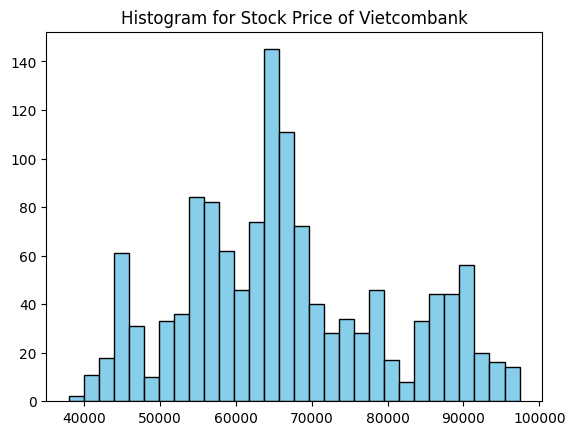
\includegraphics[width=1\textwidth]{resources/chapter-3/newdata/Histogram_Vietcombank.png}
    \caption{VCB stock price's histogram}
    \label{fig:vcb_histogram}
    \end{minipage}
\end{figure}

\subsection{Công cụ}
Trong nghiên cứu của chúng tôi, chúng tôi đã sử dụng các công cụ phân tích thống kê khác nhau trong Python để hiểu rõ hơn dữ liệu và đưa ra những kết luận ý nghĩa. Các công cụ này, bao gồm numpy, pandas, sklearn và matplotlib.pyplot, đã giúp chúng tôi khám phá ra những phát hiện đáng chú ý. Để biết kết quả chi tiết, vui lòng xem bảng mô tả và biểu đồ được cung cấp.
% end hoang

\subsection{Tỷ lệ phân chia tập dữ liệu}
Trong đồ án, phân chia dữ liệu thành hai tập: tập train và tập test theo các tỷ lệ 7:3, 8:2, 9:1. Tỷ lệ tiêu chuẩn là 7:3, tức là sử dụng 70\% dữ liệu cho việc train và 30\% cho việc test. Tỷ lệ này thường được sử dụng bởi vì với một bộ dữ liệu lớn và cần đạt được độ chính xác cao trong đánh giá mô hình, tỷ lệ 7:3 có thể tận dụng tối đa thông tin từ dữ liệu train và với một tập test chiếm 30\% trong tỷ lệ này, vẫn còn đủ dữ liệu để đánh giá hiệu quả của mô hình một cách đáng tin cậy. Bên cạnh đó, tỷ lệ 8:2 được coi là tỷ lệ tốt nhất cho việc phân chia tập train và tập test, trong đó sử dụng 80\% dữ liệu cho việc train và 20\% cho test. Tỷ lệ này thường được sử dụng khi bộ dữ liệu có kích thước lớn và tỷ lệ 8:2 sẽ giúp mô hình được train với nhiều thông tin hơn từ dữ liệu. Với một tập test chiếm 20\% quy mô, vẫn còn một lượng đáng kể dữ liệu để đánh giá hiệu quả của mô hình. Điều này giúp đảm bảo tính tin cậy và đại diện của kết quả đánh giá. Cuối cùng, tỷ lệ 9:1 có nghĩa là 90\% dữ liệu được sử dụng cho train, 10\% cho test. Tỷ lệ train gần với test sẽ giúp mô hình học được nhiều thông tin hơn từ tập huấn luyện và đánh giá hiệu quả tốt trên tập kiểm tra.

\subsection{Các chỉ số đánh giá mô hình}
Để đánh giá độ chính xác của các mô hình, chúng tôi sử dụng ba tham số là Mean Absolute Error (MAE), Mean Absolute Percentage Error (MAPE) và Root Mean Squared Error (RMSE). Thuật toán có giá trị thấp nhất trong ba thuật toán sẽ có độ chính xác tốt nhất. Dưới đây là công thức cho MAE, MAPE và RMSE.
\\ \\ \\  % =)))) suyt
\par
\textbf{RMSE} (Root Mean Squared Error) là một thước đo hiệu suất hoặc độ chính xác của một mô hình dự báo, được tính bằng cách lấy căn bậc hai của trung bình bình phương sai số giữa các giá trị dự đoán và các giá trị thực tế.
\[
\text{RMSE} = \sqrt{\frac{1}{n} \sum_{i=1}^{n} (y_i - \hat{y}_i)^2}
\]
\par
\textbf{MAPE}  (Mean Absolute Percent Error), còn được gọi là độ lệch phần trăm tuyệt đối trung bình (MAPD), là thước đo độ chính xác dự đoán của phương pháp dự báo trong thống kê. Nó thường biểu thị độ chính xác dưới dạng tỷ lệ được xác định bởi công thức:
\[
\text{MAPE} = \frac{1}{n} \sum_{i=1}^{n} \left| \frac{y_i - \hat{y}_i}{y_i} \right| \times 100
\]
\par
\textbf{MAE} (Mean Absolute Error) là một thước đo hiệu suất hoặc độ chính xác của một mô hình dự báo, được đo bằng cách tính trung bình giá trị tuyệt đối của sai số giữa giá trị thực tế và giá trị dự đoán.
\[
\text{MAE} = \frac{1}{n} \sum_{i=1}^{n} |y_i - \hat{y}_i|
\]